\documentclass[11pt,a4paper,onecolumn]{article}

\usepackage[margin=1in]{geometry}
\usepackage{amsmath,amssymb,amsthm}
\usepackage{bm}
\usepackage{booktabs}
\usepackage{hyperref}
\usepackage{enumitem}
\usepackage{xcolor}
\usepackage{graphicx}
\usepackage{array}
\usepackage{mathtools}
\usepackage[numbers,sort&compress]{natbib}

\newcommand{\R}{\mathbb{R}}
\newcommand{\E}{\mathbb{E}}
\newcommand{\tr}{\operatorname{tr}}
\newcommand{\argmax}{\operatorname*{arg\,max}}
\newcommand{\argmin}{\operatorname*{arg\,min}}
\newcommand{\Phizero}{\Phi_0}
\newcommand{\bb}{\bm{b}}
\newcommand{\bx}{\bm{x}}
\newcommand{\bc}{\bm{c}}
\newcommand{\bs}{\bm{s}}
\newcommand{\by}{\bm{y}}

\DeclareMathOperator*{\argmaxop}{\arg\max}

\title{Adaptive Sensing beyond Non-Adaptive Information Bounds:\\
       End-to-End Co-Design of Hardware, Policy, and Inference}
\author{Z.\ Lin$^{1,*}$ \emph{et~al.}\\[2pt]
\small $^1$Affiliation\quad $^*$Corresponding author}
\date{\today}

\begin{document}
\maketitle

\begin{abstract}
Real reconfigurable sensors are continuous physical hardware \emph{plus} a measurement operator that adapts to data.  End-to-end optics co-designs the first half; adaptive-sensing POMDP theory optimizes the second.  We formulate \emph{joint dynamic programming} (joint-DP) over the continuous hardware $\bc$ and a Bellman-optimal adaptive policy $\pi$, enabled by an envelope-theorem gradient that removes the policy Jacobian from the outer loop, and a relaxation hierarchy that scales from exact dynamic programming to Gaussian-posterior surrogates on $10^5$-pixel topologies.  Crucially, joint-DP delivers strictly better deployed performance than the classical workflow of selecting $\bc$ to maximize a prior-averaged, fixed-schedule information functional (mutual information, expected-Fisher log-determinant, Expected Value of Perfect Information) and attaching an adaptive policy afterwards.  On a radar beam-search POMDP, classical information-bound-guided geometry selection loses $2.8\times$ in attainable adaptive value to the joint-DP optimum.  On a superconducting-qubit flux sensor, joint-DP co-design reduces deployed mean-squared error by $13.4\%$ at $z{=}{+}11.5\sigma$ over the joint Bayesian Cram\'er--Rao baseline.  A $90{,}000$-pixel photonic metasensor co-designed via the Bayesian Fisher-information-matrix surrogate demonstrates the framework at scale.  For any sensor whose hardware is designed once but whose policy runs forever, joint $(\bc, \pi)$ optimization is the minimum principled procedure.
\end{abstract}

\tableofcontents

%===============================================================================
\section{Introduction}
\label{sec:intro}
%===============================================================================

A sensor is physical hardware paired with a rule for what to measure next.  Today these two halves are designed separately: the hardware by inverse design and end-to-end optics~\cite{sitzmann2018e2e, chang2019diffractive, metzler2020deep, tseng2021metalens, kellman2019microscopy, heide2014flex, antipa2018diffusercam, bhargava2024topology, lin2019overlapping, lin2018topology, lin2021e2e, christiansen2021fullwave, molesky2018inverse, jensen2011topology, fan2020freeform, wang2018reconfigurable}, the measurement rule by adaptive sensing and sequential Bayesian experimental design~\cite{kaelbling1998pomdp, smallwood1973sondik, sondik1971optimal, kreucher2005kastella, hero2011survey, castanon2008stochastic, chen2015adaptive, krause2005near, lindley1956measure, huan2016sequential, shen2023bayesian, alexanderian2021optimal, chaloner1995bayesian}.  Each community optimizes its own half against the other's default, a textbook setup for a joint optimum that nobody reaches.

The separation is historical rather than technical.  On the hardware side, computational inverse design now routinely reaches the electromagnetic performance bounds of the underlying scattering problem, but the downstream reconstruction it co-optimizes against is typically a single-shot feed-forward network with no concept of ``what should I measure next given what I have already seen?''.  On the policy side, adaptive sensing built on partially-observable Markov decision processes (POMDPs) and on Bayesian optimal experimental design (OED) constructs multi-step measurement rules with formal optimality guarantees, but treats the physical hardware as immutable.  Several near-relatives live in the intersection without closing it: cognitive radar adapts the waveform on a fixed antenna~\cite{bell2015cognitive, haykin2006cognitive, greco2018cognitive, bouhou2025cognitive}, Kitaev-style quantum phase estimation adapts the pulse sequence on a fixed circuit~\cite{giovannetti2006quantum, braunstein1994sld, paris2009quantum, caves1981quantum, danilin2024scqubit, kitaev1995qpe, braverman2019slowing}, programmable-metasurface imaging adapts the reconstruction on a fixed scattering medium~\cite{yurduseven2017printed, imani2020review}, and variational quantum sensing parametrizes the probe through a trainable neural ansatz rather than a geometric topology~\cite{pirandola2018advances, degen2017sensing}.  None of these treats continuous physical geometry and a multi-step Bellman-optimal measurement policy as co-equal design variables in a single optimization.

Closing this gap requires a framework that (a) is cleanly defined across discrete and continuous state spaces, (b) admits a tractable outer gradient with respect to the physical geometry, and (c) offers a hierarchy of relaxations scaling from exact dynamic programming on small POMDPs to high-dimensional continuous hardware inverse design.  We supply all three, and call the procedure \emph{joint dynamic programming}, or \emph{joint-DP}: a single optimization that treats the continuous hardware $\bc$ and the Bellman-optimal adaptive policy $\pi$ as co-equal decision variables, with $\pi$ re-solved by dynamic programming at each outer iterate in $\bc$.  To our knowledge, this is the first formulation in which continuous physical hardware and a multi-step Bellman-optimal adaptive policy are co-designed as a single optimization problem.

Joint-DP improves on the two natural baselines that bracket the problem, on benchmarks where exact comparison is tractable.  The adaptive-sensing POMDP literature runs the Bellman DP at fixed, manufacturer-specified hardware; joint-DP strictly generalizes this by co-optimizing $\bc$ under the adaptive policy, yielding a $123\times$ deployed-MSE improvement on the photonic metasensor of Case Study~C over a non-co-designed baseline.  The OED and physics-of-bounds literatures select $\bc$ to maximize a prior-averaged, fixed-schedule information functional (mutual information, expected-Fisher log-determinant, Expected Value of Perfect Information) and attach an adaptive policy afterwards; on the radar POMDP of Case Study~A the information-functional-maximizing $\bc$ loses a factor of $2.8\times$ in attainable adaptive value to the joint-DP optimum, and on the superconducting-qubit flux sensor of Case Study~B the joint Bayesian Cram\'er--Rao fixed-schedule baseline loses $13.4\%$ in deployed Bayesian MSE ($z=+11.5\sigma$).  The performance gaps are first-order in engineering terms.

\subsection{Contributions}

\begin{enumerate}[leftmargin=2em]
\item \textbf{Unified formulation.}  We identify a \emph{family} of pointwise scalar rewards $\Phi(\bx, \bs, \bc)$ that fit the same joint-$(\bc, \pi)$ Bellman machinery.  Three canonical members are (i) the mutual-information-aligned $\Phi_{\text{MI}}$ following Lindley~\cite{lindley1956measure}, (ii) the Bayesian mean-squared-error aligned $\Phi_{\text{Var}}$ tied to the deployment metric by the tower law of variance, and (iii) the Fisher-information aligned $\Phi_{\log J}$ following Cram\'er--Rao~\cite{cramer1946mathematical, rao1945information}.  Each reward picks out a different operating point; choosing $\Phi$ is a modeling commitment determined by the problem's regime.
\item \textbf{Structural insight.}  The envelope theorem of Milgrom and Segal~\cite{milgrom2002envelope} eliminates the policy Jacobian $\partial \pi^\star / \partial \bc$ from the outer geometry gradient.  This makes the joint optimization tractable even when the inner Bellman solver is approximate, and cleanly separates the \emph{algorithmic} cost of policy iteration from the \emph{physical} cost of simulating hardware.
\item \textbf{Quantitative findings, from two complementary angles.}  On a radar beam-search benchmark solved by exact enumeration and backward induction, the argmax of the prior-averaged \emph{ignorance gap} $\E[\mathrm{IG}](\bc)$ (the classical Expected Value of Perfect Information, an upper bound on adaptive gain over the best fixed schedule) loses a factor of $2.8\times$ in attainable adaptive value $V_{\text{adaptive}}$ to the joint-DP optimum.  On a continuous-state superconducting-qubit flux sensor, joint-DP co-design with $\Phi_{\text{Var}}$ reduces the deployed Bayesian mean-squared error by a statistically significant $13.4\%$ ($z = +11.5\sigma$) relative to the joint Bayesian Cram\'er--Rao fixed-schedule baseline~\cite{vantrees2007bayesian, tichavsky1998posterior}.  The 2.8$\times$ gap is the pedagogical payoff for the adaptive-sensing community; the 13.4\% MSE reduction is the engineering payoff for the hardware-metrology community.
\item \textbf{Portability across scales.}  A principled relaxation hierarchy extends the framework from the exact-DP discrete POMDP through Gaussian-posterior extended-Kalman-filter surrogates, with each rung's failure mode catalogued explicitly.  A 90{,}000-pixel photonic metasensor co-designed via the Bayesian Fisher-information-matrix surrogate demonstrates the framework at a scale $10^{4}\times$ beyond what exact Bellman dynamic programming admits.
\end{enumerate}

\subsection{Relation to prior work}

The components of our framework are individually well-established: exact Bellman DP for POMDPs~\cite{bellman1957dynamic, sondik1971optimal, smallwood1973sondik}; mutual information as an experimental-design reward (Lindley~\cite{lindley1956measure}); end-to-end optical co-design with learned reconstruction, including information-reward end-to-end imaging by Waller and collaborators~\cite{kellman2019physics, muthumbi2019learned, bostan2018deep, kellman2020datadriven}; the envelope/Danskin theorem~\cite{milgrom2002envelope, danskin1966theory}; Expected Value of Perfect Information as a classical decision-theoretic quantity~\cite{howard1966decision, raiffa1961applied}.  The joint optimization of \emph{continuous} physical hardware with a \emph{multi-step Bellman-optimal} adaptive policy is not standard in any of these: end-to-end optics uses one-step reconstructions, adaptive sensing fixes the hardware, and the EVPI/IG line does not treat continuous physical geometry as a first-class design variable.  Each ingredient is classical; the novelty is their synthesis --- a single joint optimization over continuous physical hardware and a multi-step Bellman-optimal adaptive policy, with the envelope theorem as the enabling identity on the outer gradient.

Our framework sits downstream of, and is complementary to, the recent program on fundamental limits to light--matter interaction via convex-duality and T-matrix methods~\cite{miller2016fundamental, miller2023bounds, chao2022maximum, molesky2020tmatrix, molesky2020hierarchical, molesky2020bounds, kuang2020maximal, strekalov2022bounds, gustafsson2020upper, schab2020bounds, strekalov2020bounds, molesky2019global, venkataram2020fundamental, jelinek2021upper}: those bounds certify whether a target is achievable by \emph{any} passive medium; we select the $\bc$ that realizes it along with the policy that consumes it.  Likewise for the quantum Fisher information program on wave and photon scattering~\cite{rotter2017light, bouchet2021maximum, carrington2020fisher, defienne2021coincidence, tsang2016quantum, tsang2017ziv, tsang2019resolving}: our $\Phi_{\log J}$ choice in the Gaussian-posterior regime is the Bayesian analog of the maximum-Fisher-information-state object; outside that regime it shares the stage with alternative scalar rewards chosen by the problem's deployment metric.

\subsection{Organization}

The paper builds up from formulation to evidence.  Section~\ref{sec:setup} states the joint-$(\bc, \pi)$ optimization and develops the family of pointwise scalar rewards $\Phi$.  Section~\ref{sec:decomposition} introduces the value decomposition and the ignorance gap.  Section~\ref{sec:envelope} derives the envelope-theorem outer gradient; Section~\ref{sec:hierarchy} catalogs the relaxation hierarchy.  Sections~\ref{sec:radar}, \ref{sec:scqubit}, and~\ref{sec:photonic} are the three case studies (discrete POMDP; continuous-state qubit sensor; high-dimensional photonic metasensor).  Sections~\ref{sec:discussion}--\ref{sec:conclusion} discuss limitations and conclude.

%===============================================================================
\section{Problem setup and the scalar-reward family}
\label{sec:setup}
%===============================================================================

\subsection{Sensor model}

A \emph{sensor} in this paper is a tuple $(\bc, \pi)$ where $\bc \in \mathcal{C} \subseteq \R^{d_c}$ is a continuous \emph{physical geometry} fixed at manufacturing time (the flux-bias and readout-line mutual inductances of a SQUID loop, the permittivity distribution of an inverse-designed metasurface, the elements of a phased-array antenna), and $\pi: \mathcal{B} \to \mathcal{S}$ is a \emph{measurement policy} that maps the current belief $\bb \in \mathcal{B}$ over the unknown state $\bx \in \mathcal{X}$ to an action $\bs \in \mathcal{S}$.  At each step $k \in \{1, \ldots, K\}$ the policy emits an action $\bs_k = \pi(\bb_k)$, whose execution produces a \emph{measurement} $\by_k \in \mathcal{Y}$ drawn from the likelihood
\begin{equation}
  \by_k \;\sim\; p(\by_k \mid \bx, \bs_k;\, \bc),
  \label{eq:likelihood}
\end{equation}
where $\mathcal{Y}$ is the measurement space specified by the physical readout (discrete detector counts in a photon-starved regime, photon clicks in a Ramsey sequence, real-valued voltages from a homodyne detector, etc.) and $\bc$ parametrizes the likelihood through its physical forward model (Maxwell's equations, circuit Hamiltonian dynamics, Schr\"odinger evolution with pulse shaping, etc.).  For non-adaptive (``fixed-schedule'') policies $\pi$ is a constant function of the belief; for adaptive policies $\pi$ depends on the history $\mathcal{F}_{k-1} = \{\bs_{1:k-1}, \by_{1:k-1}\}$ through the posterior $\bb_k = p(\bx \mid \mathcal{F}_{k-1};\, \bc)$.  We write $K$ for the \emph{horizon} --- the total number of measurement steps the operator is budgeted before an estimate of $\bx$ is reported, which may be limited by coherence time in a quantum sensor, by integration-time budget in a radar search, or by throughput requirements in an imaging pipeline --- $p_0(\bx)$ for the prior, and reserve $\pi^\star(\bc)$ for the Bellman-optimal policy at fixed $\bc$.  Inner expectations are over observations $\by$ with $\bx, \bc$ held fixed; outer expectations are over the prior $p_0$.

\subsection{Joint optimization statement}

A \emph{joint co-design objective} is any scalar functional of the hardware-policy pair,
\begin{equation}
  V(\bc, \pi) \;=\; \E_{\bx \sim p_0}\, \E_{\by_{1:K} \mid \bx, \pi, \bc}\!\bigl[\, \Phi(\bx, \bs_{1:K}^{\pi}, \bc) \,\bigr],
  \label{eq:V_def}
\end{equation}
where $\Phi: \mathcal{X} \times \mathcal{S}^K \times \mathcal{C} \to \R$ is a user-specified \emph{pointwise reward}: ``pointwise'' in the sense that $\Phi$ is evaluated at each realization of the true state $\bx$, action sequence $\bs_{1:K}$, and hardware $\bc$ separately, before any averaging over the prior.  Aggregate objectives (Bayesian mean-squared error, mutual information, log-determinant of an expected Fisher matrix) are recovered by taking the expectations in Equation~\eqref{eq:V_def}.  We correspondingly use ``pointwise MSE'' for the state-conditional mean-squared error $\E_{\by \mid \bx}[(\hat\bx - \bx)^2]$, which is an $\bx$-dependent scalar, as opposed to the aggregate Bayesian MSE which is its prior average.  The joint hardware--policy optimization solves
\begin{equation}
  (\bc^\star, \pi^\star) \;=\; \argmax_{\bc \in \mathcal{C},\; \pi \in \Pi}\; V(\bc, \pi).
  \label{eq:joint_opt}
\end{equation}
Equation~\eqref{eq:joint_opt} is the sole formal statement in the paper; what varies across applications is only the choice of~$\Phi$.  Two degenerate cases recover classical programs: $\Pi = \{\text{constant policies}\}$ with $\Phi$ minus a reconstruction loss recovers \textbf{end-to-end optics}~\cite{sitzmann2018e2e, chang2019diffractive}; $\mathcal{C} = \{\bc_0\}$ (fixed hardware) with any $\Phi$ recovers \textbf{adaptive sensor management}~\cite{kaelbling1998pomdp, kreucher2005kastella}.  Their pairing is the content of this paper.

For the posterior-mean estimator on continuous $\bx$, the tower-law identity $\E[(\hat\bx_{\text{pm}} - \bx)^2] = \E[\mathrm{Var}(\bx \mid \bb_K)]$ makes the Bayesian MSE a special case of $V(\bc, \pi)$ with $\Phi = -\mathrm{Var}(\bx \mid \bb_K)$.  Section~\ref{sec:phi_family} develops this and two alternative $\Phi$ choices used by the other case studies.

%===============================================================================
\subsection{The scalar-reward family $\Phi$}
\label{sec:phi_family}

Three canonical choices for $\Phi$ emerge naturally from three different bodies of theory.  In each case $\Phi$ is a deterministic function of $(\bx, \bs_{1:K}, \bc)$; any expectation over the measurement trajectory $\by_{1:K}$ that appears in the definition is baked in, so that the outer objective $V(\bc, \pi) = \E_{\bx, \by}[\Phi]$ of Equation~\eqref{eq:V_def} is a single expectation over the prior and the data.

\paragraph{Mutual-information-aligned reward $\Phi_{\text{MI}}$.}  Following the Shannon--Lindley line~\cite{shannon1948mathematical, lindley1956measure} through Chaloner--Verdinelli~\cite{chaloner1995bayesian}, Sebastiani--Wynn~\cite{sebastiani2000optimal}, and the adaptive sensor-management literature~\cite{kreucher2005kastella, hero2011survey},
\begin{equation}
  \Phi_{\text{MI}}(\bx, \bs, \bc) \;=\; \E_{\by\mid\bx, \bs, \bc}\!\bigl[\ln|\mathrm{supp}(\bb_K)| - H(\bb_K)\bigr],
\end{equation}
the expected negative entropy of the terminal belief $\bb_K$ at state $\bx$.  Averaging over the prior gives $\E_{\bx}[\Phi_{\text{MI}}] = I(\bx; \by_{1:K} \mid \bs, \bc)$, the mutual information.  This is the reward of choice for discrete-state problems where MSE is undefined or dominated by 0/1 classification loss~\cite{castanon2008stochastic}, and for any problem in the large-$K$ Bernstein--von Mises regime~\cite{vaart2000asymptotic, clark2021bvm} where the Gaussian-posterior approximation makes MI monotone in MSE.  The photonic and quantum-sensing communities have developed extensive machinery for \emph{upper bounds} on achievable mutual information given physical constraints (reciprocity, passivity, energy); our framework consumes those bounds as constraints on the feasible set $\{\Phi_{\text{MI}}(\cdot, \cdot, \bc) : \bc \in \mathcal{C}\}$ rather than re-deriving them.

\paragraph{Bayesian-MSE-aligned reward $\Phi_{\text{Var}}$.}  Inheriting from the Bayesian Cram\'er--Rao tradition~\cite{vantrees2007bayesian} and the posterior-variance-minimization line of Bayesian optimal experimental design~\cite{chaloner1995bayesian, pronzato2010optimal}, the tower law of variance
\begin{equation}
  \E_{\bx, \by_{1:K}}\!\left[(\hat\bx_{\text{pm}} - \bx)^2\right]
  \;=\; \E_{\by_{1:K}}\!\left[\mathrm{Var}(\bx \mid \by_{1:K})\right]
\end{equation}
(with $\hat\bx_{\text{pm}}$ the posterior mean) motivates
\begin{equation}
  \Phi_{\text{Var}}(\bx, \bs, \bc) \;=\; \E_{\by\mid\bx, \bs, \bc}\!\bigl[-\mathrm{Var}(\bx \mid \bb_K)\bigr],
\end{equation}
for which the outer objective $V(\bc, \pi)$ equals $-1\times$ the deployed Bayesian MSE exactly.  The joint-DP optimum of this reward is literally the \emph{MSE-optimal} adaptive policy at fixed $\bc$, without any asymptotic approximation.  For continuous-state, finite-$K$ problems with bounded-support priors, where the Bernstein--von Mises regime is not reached, $\Phi_{\text{Var}}$ strictly dominates $\Phi_{\text{MI}}$ as an MSE anchor.  The tower-law identity is textbook; its use as a joint-DP terminal reward in the present hardware-policy setting is new.

\paragraph{Fisher-information-aligned reward $\Phi_{\log J}$.}  Inheriting from the classical Fisher-information-matrix tradition~\cite{cramer1946mathematical, rao1945information, berger1985statistical} and its Bayesian extension~\cite{vantrees2007bayesian, tichavsky1998posterior}, and applicable to continuous $\bx$ with a Gaussian-posterior surrogate,
\begin{equation}
  \Phi_{\log J}(\bx, \bs, \bc) \;=\; \tfrac{1}{2} \log\det J_N(\bx, \bs_{1:K}, \bc),
\end{equation}
where $J_N$ is the accumulated Fisher information matrix at true $\bx$.  The outer expectation is the log-determinant of the Bayesian Fisher information matrix~\cite{pilanci2015randomized, chaloner1995bayesian}, with $J_N^{-1}$ the Bayesian CRB.  In the Gaussian-posterior regime $\Phi_{\log J}$ agrees with $\Phi_{\text{Var}}$ up to log-transforms.  Outside that regime (biased estimators, bounded priors, small $K$), $\Phi_{\log J}$ retains an asymptotic CRB interpretation while losing its direct link to finite-sample MSE.  It is the natural reward for high-dimensional continuous problems where the full Bellman DP is intractable and the Gaussian surrogate is the cheapest defensible relaxation.  The quantum-Fisher-information program on wave and photon scattering~\cite{bouchet2021maximum, tsang2016quantum, rotter2017light, carrington2020fisher} and the photonic information-bound program on scattering-matrix extremization~\cite{miller2016fundamental, miller2023bounds, chao2022maximum, molesky2020tmatrix, molesky2020hierarchical} establish upper bounds on $\det J_N$ over admissible $\bc$; they tell us what $\sup_{\bc} \det J_N$ is, and our framework tells us which $\bc$ and which policy realize it jointly.

\subsection{Comparison and operational guidance}
\label{sec:phi_compare}

\begin{table}[h]
\centering
\caption{Three natural pointwise scalar rewards, their operational semantics, and their alignment with finite-$K$ MSE.}
\label{tab:phi_family}
\begin{tabular}{@{}llll@{}}
\toprule
reward & terminal expression & community & tied to pointwise MSE? \\
\midrule
$\Phi_{\text{MI}}$  & $\ln|\mathrm{supp}(\bb_K)| - H(\bb_K)$            & sensor management, sOED & asymptotic only \\
$\Phi_{\text{Var}}$ & $-\mathrm{Var}(\bx \mid \bb_K)$                   & Bayesian estimation     & \textbf{directly, by tower law} \\
$\Phi_{\log J}$     & $\tfrac{1}{2}\log\det J_N(\bx, \bs, \bc)$         & Fisher info, PCRB       & asymptotic only \\
\bottomrule
\end{tabular}
\end{table}

The three rewards agree asymptotically under Bernstein--von Mises but diverge at finite horizons.  Case~Study~B below reports a 17\% absolute gap between the optima found under $\Phi_{\text{MI}}$ and $\Phi_{\text{Var}}$ on the same scqubit benchmark at $K=3$, a quantitative demonstration that the choice of $\Phi$ matters operationally.  We accordingly present the paper's machinery as reward-agnostic: the user picks $\Phi$ based on the problem's state space, horizon, and deployment metric, and the envelope-theorem outer gradient of Section~\ref{sec:envelope} derives identically from any of them.

%===============================================================================
\section{Value decomposition and the ignorance gap}
\label{sec:decomposition}
%===============================================================================

For any choice of $\Phi$, the outer objective $V(\bc, \pi)$ admits a four-functional decomposition that is useful for both intuition and diagnostics.  The decomposition is standard in sequential Bayesian experimental design~\cite{huan2016sequential, shen2023bayesian} and was used in the radar sensor-management literature under the name ``oracle value'' of perfect information~\cite{kreucher2005kastella, kastella1997discrimination}; we restate it in the $\Phi$-agnostic form used in the rest of the paper.

\subsection{Four functionals}
\label{sec:four_functionals}

\begin{align}
V_{\text{oracle}}(\bx, \bc) &= \max_{\bs_{1:K}} \Phi(\bx, \bs_{1:K}, \bc), \label{eq:Voracle}\\
V_{\text{fixed}}(\bc)       &= \max_{\bs_{1:K}} \E_{\bx}\!\bigl[\Phi(\bx, \bs_{1:K}, \bc)\bigr], \label{eq:Vfixed}\\
V_{\text{adaptive}}(\bc)    &= \max_{\pi \in \Pi} \E_{\bx} \E_{\by\mid\bx, \pi, \bc}\!\bigl[\Phi(\bx, \bs_{1:K}^\pi, \bc)\bigr], \label{eq:Vadaptive}\\
\E[\mathrm{IG}](\bc)        &= \E_{\bx}[V_{\text{oracle}}(\bx, \bc)] - V_{\text{fixed}}(\bc). \label{eq:EIG}
\end{align}

The functional $V_{\text{oracle}}(\bx, \bc)$ is the value attained by a \emph{clairvoyant} sensor that knows the true $\bx$ and picks the best fixed schedule for it; its prior average is an oracle upper bound.  $V_{\text{fixed}}(\bc)$ is the best non-adaptive schedule.  $V_{\text{adaptive}}(\bc)$ is the best adaptive policy, which is the quantity the user ultimately deploys.  $\E[\mathrm{IG}](\bc)$, the \emph{expected ignorance gap} or \emph{expected value of perfect information} (EVPI)~\cite{howard1966decision, raiffa1961applied}, is a well-defined scalar functional of $\bc$ that measures how much adaptive slack exists at that geometry.

\subsection{The case for joint hardware--policy co-design}
\label{sec:codesign_case}

The quantity the user deploys is $V_{\text{adaptive}}(\bc)$: the value attained by the best adaptive policy at the chosen hardware.  Two facts make it a function of $\bc$ that cannot be maximized piecewise.

\paragraph{Fact 1: adaptation extracts real value at most geometries.}  A fixed schedule commits all $K$ measurements in advance, before any data has arrived.  An adaptive policy sees each outcome as it happens and re-routes subsequent measurements accordingly: effort that would have been wasted confirming something the data has already settled gets redirected toward parts of the state space that remain ambiguous.  In an imaging problem this is the difference between a fixed raster scan and one that zooms in on the suspected region; in a qubit-flux sensor it is the difference between a fixed Ramsey delay ladder and one that shortens $\tau$ when the posterior is broad (to avoid phase-wrapping ambiguity) and lengthens $\tau$ once the flux is roughly localized.  The resulting \emph{adaptive gain} $V_{\text{adaptive}}(\bc) - V_{\text{fixed}}(\bc)$ is typically strictly positive and often sizable.

\paragraph{Fact 2: the adaptive gain depends nontrivially on $\bc$.}  A hardware configuration that maximizes $V_{\text{fixed}}$ is not in general the hardware that maximizes $V_{\text{adaptive}}$: a geometry good for blind schedules is good because its expected measurements are individually informative on average, and that property tends to leave little room for outcome-dependent re-routing.  Conversely, a geometry with very large \emph{oracle} value (what a clairvoyant sensor with perfect knowledge of $\bx$ could achieve) may put so much of that value out of reach of any policy that only sees past data that the realizable adaptive value is actually small.  The geometry that deploys well under an adaptive policy is an \emph{interior} geometry, one that neither is over-tuned to blind schedules nor relies on clairvoyance; this optimum is not located by examining $V_{\text{fixed}}$ or $V_{\text{oracle}}$ separately.

\paragraph{Consequence: the two layers cannot be solved in sequence.}  One cannot pick $\bc$ first (by any single-functional criterion) and then pick $\pi$, because the criterion for a good $\bc$ depends on which $\pi$ will follow.  Joint optimization of $(\bc, \pi)$ is necessary; the rest of the paper is about making it tractable.  Section~\ref{sec:envelope} gives the envelope-theorem identity that decouples the \emph{gradient computation} from the inner-policy solve even when the two quantities themselves do not decouple, so that an outer-loop optimizer can climb $V_{\text{adaptive}}(\bc)$ with a single Bellman solve per iteration.

\subsection{A natural shortcut via EVPI, and why it fails}
\label{sec:evpi_shortcut}

Before committing to the joint solve, it is worth asking whether some cheaper criterion identifies the right $\bc$.  The four-functional decomposition suggests a tempting candidate: the EVPI.  Chaining the inequalities
\begin{equation}
V_{\text{fixed}}(\bc) \;\le\; V_{\text{adaptive}}(\bc) \;\le\; \E_{\bx}[V_{\text{oracle}}(\bx, \bc)]
\label{eq:chain}
\end{equation}
(fixed schedules are a subset of adaptive policies, and no policy beats the clairvoyant oracle) gives the EVPI upper bound
\begin{equation}
V_{\text{adaptive}}(\bc) - V_{\text{fixed}}(\bc) \;\le\; \E[\mathrm{IG}](\bc).
\label{eq:evpi}
\end{equation}
Since $V_{\text{oracle}}$ and $V_{\text{fixed}}$ are obtainable by direct schedule enumeration, $\E[\mathrm{IG}](\bc)$ is cheap to compute in any setting where the schedule space is enumerable, unlike $V_{\text{adaptive}}(\bc)$ which requires a full backward-induction DP.  So one might hope to pick $\bc^{\text{EVPI}} = \argmax_{\bc} \E[\mathrm{IG}](\bc)$ and proceed.

This shortcut fails empirically.  The critical observation, which we back up quantitatively in Section~\ref{sec:radar}, is that the bound in~\eqref{eq:evpi} is typically slack \emph{and its slackness pattern is non-monotone in $\bc$}:
\begin{equation}
\argmax_{\bc} \,\E[\mathrm{IG}](\bc) \;\;\ne\;\; \argmax_{\bc} V_{\text{adaptive}}(\bc).
\label{eq:argmax_mismatch}
\end{equation}
The geometry with the largest in-principle adaptive gain, as measured by EVPI, is typically a geometry where most of that gain is unreachable in practice.  Extreme geometries (a very narrow beam, a near-isotropic beam) produce high EVPI because the oracle's advantage over any blind fixed schedule is enormous; but the adaptive policy, which does not know $\bx$, cannot replicate the oracle's strategy and captures only a small fraction of the nominal headroom.  Interior geometries, by contrast, have a modest EVPI ceiling but let the adaptive policy capture a larger fraction of it, which is what ultimately matters.  On a canonical radar benchmark (Case~Study~A, Section~\ref{sec:radar}), $\bc^{\text{EVPI}}$ loses a factor of $2.8\times$ in attainable $V_{\text{adaptive}}$ to the joint-DP optimum.  The joint solve is unavoidable.

\subsection{EVPI's remaining roles}

Although EVPI cannot replace the joint solve as a design criterion, it retains three useful roles:
\begin{enumerate}[nosep]
\item \textbf{A pre-screen when the full joint DP is prohibitive but schedule enumeration is tractable.}  $\E[\mathrm{IG}](\bc)$ depends only on $V_{\text{oracle}}$ and $V_{\text{fixed}}$; its cheapness is inherited from the cheapness of those enumerations (small discrete action sets or low-dimensional continuous actions on a reasonable grid), and evaporates when schedule enumeration itself becomes the bottleneck.
\item \textbf{Post-hoc interpretation.}  After solving the joint problem, $\E[\mathrm{IG}](\bc^\star)$ quantifies the headroom between the attained adaptive value and the oracle ceiling, indicating where further gains might come from (longer horizon, richer action set).
\item \textbf{Diagnostic lens on the slackness pattern.}  When $\argmax_{\bc} \E[\mathrm{IG}]$ and $\argmax_{\bc} V_{\text{adaptive}}$ disagree, the disagreement structure exposes the physics: extreme geometries leave the most adaptive headroom on the table, and interior geometries capture more of a smaller ceiling.  Section~\ref{sec:radar} develops this in detail.
\end{enumerate}

%===============================================================================
\section{Envelope-theorem gradient for the outer loop}
\label{sec:envelope}
%===============================================================================

\subsection{Statement}

Let $\pi^\star(\bc) = \argmax_{\pi \in \Pi} V(\bc, \pi)$ be the optimal policy at hardware $\bc$.  The joint-optimal geometry solves
\begin{equation}
\bc^\star = \argmax_{\bc} V^\star(\bc), \qquad V^\star(\bc) \coloneqq V(\bc, \pi^\star(\bc)).
\end{equation}
A naive outer gradient requires differentiating through the policy argmax:
\begin{equation}
\frac{dV^\star}{d\bc} \;=\; \frac{\partial V}{\partial \bc}\bigg|_{\pi = \pi^\star(\bc)} \;+\; \underbrace{\frac{\partial V}{\partial \pi}\bigg|_{\pi = \pi^\star(\bc)}}_{= 0 \text{ at optimum}} \cdot \frac{d\pi^\star}{d\bc}.
\end{equation}
The second term vanishes at the optimum by the first-order optimality condition (or, in discrete-action settings, by the envelope/Danskin theorem~\cite{danskin1966theory, milgrom2002envelope, bonnans2000perturbation}).  Consequently the outer gradient is simply
\begin{equation}
\boxed{\;\frac{dV^\star}{d\bc} \;=\; \frac{\partial V(\bc, \pi^\star(\bc))}{\partial \bc}\bigg|_{\pi^\star \text{ held fixed}}.\;}
\label{eq:envelope_gradient}
\end{equation}
The policy Jacobian $d\pi^\star/d\bc$ does not appear.

\subsection{Implications for tractability}

Equation~\eqref{eq:envelope_gradient} is the workhorse of the paper.  Four consequences:
\begin{enumerate}[nosep]
\item The outer gradient requires solving the inner problem once (to obtain $\pi^\star(\bc)$) and then differentiating $V$ through the likelihood while holding the policy fixed.  This decouples the computational cost of solving the Bellman DP from the cost of computing the outer gradient.
\item When $\pi^\star(\bc)$ is computed only approximately (by deep RL, by an approximate value iteration, by a myopic one-step-lookahead), the envelope theorem still says that at the \emph{approximate} optimum, the approximate policy Jacobian's contribution to the outer gradient is first-order small.  The framework accommodates approximate inner solvers without bias.
\item The outer gradient is differentiable in $\bc$ whenever the likelihood is differentiable in $\bc$.  For photonic problems this is automatic via differentiable electromagnetic simulation~\cite{hughes2018adjoint, minkov2020inverse}; for quantum-circuit problems via differentiable Hamiltonian dynamics~\cite{khaneja2005optimal}.
\item The envelope gradient admits a simple Monte-Carlo realization: sample trajectories under $\pi^\star$, differentiate the trajectory log-likelihood times the terminal reward under $\bc$, average.  This is the pathwise REINFORCE estimator~\cite{williams1992reinforce, schulman2015pathwise} specialized to the fixed-policy case.
\end{enumerate}

\subsection{Policy iteration}

The natural outer-loop algorithm alternates Bellman solves with envelope gradient steps:
\begin{quote}
\noindent \textbf{Joint $(\bc, \pi)$ policy iteration:}
\begin{enumerate}[nosep, leftmargin=2em]
\item[1.] Initialize $\bc^{(0)}$.
\item[2.] For $t = 1, 2, \ldots$ until convergence:
  \begin{itemize}[nosep]
  \item Inner: solve $\pi^\star(\bc^{(t-1)})$ (exact DP, deep RL, myopic, etc.).
  \item Outer: $\bc^{(t)} = \bc^{(t-1)} + \eta \cdot \frac{\partial V(\bc^{(t-1)}, \pi^\star(\bc^{(t-1)}))}{\partial \bc}$ with step size $\eta$.
  \item Optionally: box-project $\bc^{(t)}$ onto the feasible set.
  \end{itemize}
\end{enumerate}
\end{quote}
Convergence to a stationary point of $V^\star$ follows from standard policy-iteration theory~\cite{puterman2014markov, bertsekas1996neuro} when the inner solver is exact; the envelope theorem extends this to approximate inner solvers provided the approximation error is $o(\eta)$.

\subsection{A note on continuous actions}

Nothing in the envelope theorem presupposes discrete actions.  For continuous $\bs$, the Bellman backup's inner maximization is a continuous optimization:
\begin{equation}
V_k(\bb) = \max_{\bs \in \mathcal{S}} \E_{\by}[V_{k+1}(T(\bb, \bs, \by))],
\end{equation}
with the terminal condition $V_K$ given by the inner expression of $\Phi$ at the terminal belief (Table~\ref{tab:phi_family}).  The $k=0$ value under the optimal policy coincides with $V(\bc, \pi^\star)$ of Equation~\eqref{eq:V_def}.
Standard tools, differential dynamic programming~\cite{jacobson1970ddp, tassa2012ddp}, sample-based tree search~\cite{silver2010monte, couetoux2011continuous}, local gradient inner optimization, HJB-PDE solutions~\cite{munos2014bandits}, apply.  The one caveat specific to our setting is that the standard count-statistic belief memoization used by discrete-action Bellman DP (Section~\ref{sec:radar}) fails for continuous actions because distinct inner-optimization candidates produce distinct child beliefs.  We handle this in Case~Study~C by using the Gaussian-posterior surrogate, in which the belief state is finite-dimensional and the Bellman backup admits a one-step-lookahead closed form; and in Case~Study~B by fine discretization of the continuous action dimension (achieving $\sim 99\%$ of the continuous performance at $\sim 10\%$ of the implementation complexity).

%===============================================================================
\section{A hierarchy of relaxations}
\label{sec:hierarchy}
%===============================================================================

The joint $(\bc, \pi)$ optimization as stated in Section~\ref{sec:setup} is exactly solvable only for small discrete POMDPs.  In practice one must relax either the inner Bellman solver, the state-space representation, or both.  We catalog five relaxation rungs, each with a clear operational regime and failure mode.

\begin{center}
\begin{tabular}{@{}lll@{}}
\toprule
rung & method & failure mode \\
\midrule
1 & Exact Bellman DP (discrete state, small $K$)        & memoization blows up for $|\mathcal{S}|^K \gtrsim 10^6$ \\
2 & Approximate DP / deep RL (discrete state, large $K$) & value-function approximation error \\
3 & Certainty equivalence (continuous state)            & ignores observation uncertainty in the policy \\
4 & Myopic Bayesian $D$-optimal                          & ignores future decisions (one-step-lookahead) \\
5 & Gaussian-trace + EKF (continuous state, high-$d_c$) & Gaussian-posterior approximation breaks near bounds \\
\bottomrule
\end{tabular}
\end{center}

The three case studies below cover rungs 1, 1, and 5 respectively.  Rungs 2--4 are consumed from the literature, POMCP~\cite{silver2010monte}, deep Q-learning for POMDPs~\cite{hausknecht2015deep}, deep RL for sensor scheduling~\cite{zhong2018deep}, Bayesian optimal experimental design with adjoint surrogates~\cite{huan2016sequential, shen2023bayesian}, myopic expected information gain~\cite{drovandi2014sequential}, and integrated into the framework via the envelope theorem without modification.

\paragraph{When each rung is the right tool.}  The right rung is the one that makes the outer loop tractable without introducing errors that invalidate the claim structure of Equation~\eqref{eq:chain}.  In practice this selects rung 1 for discrete POMDPs with $K \le 4$; rung 2 for discrete POMDPs with $K \ge 6$; rungs 3--4 for continuous states at moderate scale; rung 5 for high-dimensional continuous geometry.  The scqubit case study below is at rung 1 (continuous state, $K = 3$, exact DP with $K_\Phi$-point grid belief); the photonic case study is at rung 5.  No one rung uniformly dominates; each names its failure mode explicitly so that a practitioner can choose deliberately.

%===============================================================================
\section{Case Study A: Radar beam search (exact DP, discrete state, $\Phi_{\text{MI}}$)}
\label{sec:radar}
%===============================================================================

The radar beam-search case is the smallest non-trivial POMDP that exhibits the full $V_{\text{oracle}}/V_{\text{fixed}}/V_{\text{adaptive}}/\E[\mathrm{IG}]$ decomposition.  We present it as the pedagogical entry point to the paper's quantitative findings.

\subsection{Problem setup}

\paragraph{State.}  $\bx \in \{1, \ldots, K\}$ is a target cell on a ring, $K = 16$.  Prior $p_0(\bx) = 1/K$.

\paragraph{Action.}  At each of $N = 4$ epochs the sensor points a beam at cell $\bs_k \in \{1, \ldots, K\}$.

\paragraph{Observation.}  $\by_k \in \{0, 1\}$ (miss/detection) with Bernoulli likelihood
\begin{equation}
p(\by_k = 1 \mid \bx, \bs_k; \bc) = p_\mathrm{FA} + (p_\mathrm{D} - p_\mathrm{FA}) \cdot G_{\bc}(\theta_{\bs_k} - \varphi_{\bx}),
\end{equation}
with $p_\mathrm{D} = 0.9$, $p_\mathrm{FA} = 0.05$, cell bearings $\varphi_{\bx} = 2\pi(\bx - 1)/K$, and pointing angles $\theta_{\bs_k}$.  The geometry family is a top-hat beam parametrized by integer width $m \in \{1, \ldots, K\}$: the beam centered on cell $a$ covers all cells within a ring distance of $\lfloor m/2 \rfloor$ from $a$, giving detection probability $p_\mathrm{D}$ inside the beam and $p_\mathrm{FA}$ outside.  $m$ is the discrete design variable for the within-family sweep below.

\paragraph{Reward.}  $\Phi = \Phi_{\text{MI}}$, since the state is discrete and there is no natural MSE.

\subsection{Enumeration results}

The exact enumeration of $V_{\text{oracle}}$, $V_{\text{fixed}}$, and backward-induction $V_{\text{adaptive}}$ at $K = 16$, $N = 4$ is computationally modest (order $10^7$ elementary operations, Julia runtime $\sim 0.1$~s on a single thread).  In the narrow-beam ($m = 1$) and wide-beam ($m = 8$) regimes we obtain:

\begin{center}
\begin{tabular}{@{}lrr@{}}
\toprule
 & narrow ($m = 1$) & wide ($m = 8$) \\
\midrule
$V_{\text{oracle}}$       & $2.580$ nats & $1.923$ nats \\
$V_{\text{adaptive}}$     & $0.619$      & $1.700$      \\
$V_{\text{fixed}}$        & $0.499$      & $1.411$      \\
$\E[\mathrm{IG}]$         & $2.081$      & $0.513$      \\
realized gain $V_{\text{adaptive}} - V_{\text{fixed}}$ & $0.121$ & $0.289$ \\
EVPI saturation           & $5.8\%$      & $56.4\%$     \\
\bottomrule
\end{tabular}
\end{center}

Note the non-monotone relationship: the narrow regime has the largest $\E[\mathrm{IG}]$ (more than $4\times$ the wide regime's) but the smallest realized adaptive gain (less than half).  The narrow EVPI is ``loose'', most of the adaptive headroom is unreachable by any policy at $N = 4$, while the wide EVPI is relatively tight.

\subsection{Within-family sweep over the top-hat beam width}

Sweeping the integer beam width $m \in \{1, \ldots, K\}$ and reporting all four functionals:

\begin{center}
\begin{tabular}{@{}rrrrrrr@{}}
\toprule
$m$ & $V_{\text{oracle}}$ & $V_{\text{adaptive}}$ & $V_{\text{fixed}}$ & $\E[\mathrm{IG}]$ & realized & sat.\ \% \\
\midrule
 1 & $2.580$ & $0.619$ & $0.499$ & $\mathbf{2.081}$ & $0.121$ & $5.8$  \\
 2 & $2.580$ & $0.619$ & $0.499$ & $2.081$ & $0.121$ & $5.8$  \\
 3 & $2.293$ & $1.401$ & $1.103$ & $1.190$ & $0.299$ & $25.1$ \\
 5 & $2.081$ & $1.631$ & $1.343$ & $0.737$ & $0.287$ & $38.9$ \\
 7 & $1.924$ & $1.700$ & $\mathbf{1.411}$ & $0.513$ & $0.289$ & $56.4$ \\
\textbf{9} & $1.879$ & $\mathbf{1.704}$ & $1.401$ & $0.478$ & $\mathbf{0.303}$ & $\mathbf{63.5}$ \\
11 & $2.074$ & $1.632$ & $1.320$ & $0.754$ & $0.312$ & $41.4$ \\
13 & $2.312$ & $1.389$ & $1.041$ & $1.271$ & $0.347$ & $27.3$ \\
15 & $2.514$ & $0.611$ & $0.442$ & $2.071$ & $0.169$ & $8.1$  \\
16 & $2.514$ & $0.611$ & $0.442$ & $2.071$ & $0.169$ & $8.1$  \\
\bottomrule
\end{tabular}
\end{center}

The in-family optimum for $V_{\text{adaptive}}$ is at $m^\star = 9$ ($V_{\text{adaptive}}^\star = 1.704$ nats, saturation $63.5\%$).  $V_{\text{fixed}}$ peaks one cell earlier at $m = 7$.  Realized adaptive gain $V_{\text{adaptive}} - V_{\text{fixed}}$ peaks at $m = 13$ ($0.347$ nats).  And the ignorance gap $\E[\mathrm{IG}]$ peaks at the two \emph{extremes} $m = 1$ (narrow) and $m = 16$ (isotropic), far from any $V_{\text{adaptive}}$ or $V_{\text{fixed}}$ maximum.

\subsection{Within-family three-way comparison: EVPI picks the wrong geometry}

\begin{center}
\fbox{\parbox{0.93\textwidth}{
\textbf{Top-hat within-family three-way comparison.}
\begin{center}
\begin{tabular}{@{}lrrrrr@{}}
\toprule
$\bc$ & $\E[\mathrm{IG}]$ & $V_{\text{adaptive}}$ & $V_{\text{fixed}}$ & realized & sat. \\
\midrule
top-hat $m = 1$ (narrow extreme)            & $\mathbf{2.081}$ & $0.619$          & $0.499$          & $0.121$          & $5.8\%$           \\
top-hat $m = 16$ (isotropic extreme)        & $2.071$          & $0.611$          & $0.442$          & $0.169$          & $8.1\%$           \\
top-hat $m = 9$ (in-family optimum)         & $0.478$          & $\mathbf{1.704}$ & $\mathbf{1.401}$ & $\mathbf{0.303}$ & $\mathbf{63.5\%}$ \\
\bottomrule
\end{tabular}
\end{center}
The in-family optimum $m^\star = 9$ dominates both extremes on every actionable column: $V_{\text{adaptive}}$, $V_{\text{fixed}}$, realized gain, and saturation.  The \emph{only} column on which it is not best is $\E[\mathrm{IG}]$, where both extremes beat it by a factor of four.  An EVPI-only geometry selection would reject $m^\star = 9$ in favor of either $m = 1$ or $m = 16$, both of which realize $V_{\text{adaptive}}$ that is nearly three times worse.  This ratio, $V_{\text{adaptive}}(m = 9) / V_{\text{adaptive}}(m = 1) = 1.704 / 0.619 \approx 2.75$, is the paper's ``$2.8\times$'' quantitative headline in its cleanest form: \emph{the EVPI-argmax geometry is strictly suboptimal in attainable adaptive value by a factor of $\sim 2.75\times$ on the top-hat family at this problem size.}
}}
\end{center}

The same observation underwrites the conceptual claim of Section~\ref{sec:decomposition}: $\argmax_{\bc} \E[\mathrm{IG}](\bc) \ne \argmax_{\bc} V_{\text{adaptive}}(\bc)$, the disagreement is operationally large, and only the full joint solve picks the right geometry.

\subsection{Optimal adaptive policy structure}

The DP-optimal policy tree reveals structure beyond what the scalar values expose.  In the wide ($m = 8$) regime, the depth-2 head of the tree is:

\begin{center}
\begin{tabular}{@{}ll@{}}
\toprule
history & action \\
\midrule
$\emptyset$         & cell 1 \\
$y_1 = 0$ (miss)    & cell 4 \\
$y_1 = 1$ (detect)  & cell 13 \\
\bottomrule
\end{tabular}
\end{center}

A detection at cell 1 (which covers cells $\{14, 15, 16, 1, 2, 3, 4\}$) narrows the support to the upper ring half; step 2 at cell 13 (covering $\{10, \ldots, 16\}$) bisects that half.  This is binary search conditioned on the observation, the hallmark of adaptive value that fixed schedules cannot replicate.

%===============================================================================
\section{Case Study B: Superconducting-qubit flux sensor (exact DP, continuous state, $\Phi_{\text{Var}}$)}
\label{sec:scqubit}
%===============================================================================

Case Study A is discrete-state and has no natural MSE metric; Case Study B takes the same exact-DP machinery to a continuous-state problem where the natural deployment metric is Bayesian MSE.  The case study's central claim is the paper's \emph{operational} headline: joint-DP co-design with $\Phi_{\text{Var}}$ beats the joint Bayesian Cram\'er--Rao fixed-schedule baseline on deployed MSE, at statistical significance $z = +11.5\sigma$.

\subsection{Problem setup}

We consider the frequency-tunable transmon flux sensor of Danilin, Nugent \& Weides~\cite{danilin2024scqubit}.  The unknown is the external magnetic flux $\bx = \Phi_\mathrm{ext} \in [0, \Phi_0/2]$ threading a SQUID loop.  Ramsey interferometry at a fixed operating flux $\Phi^\star$ returns a Bernoulli outcome with likelihood
\begin{equation}
p(\by = 1 \mid \bx, \tau; \bc) = \tfrac{1}{2} + \tfrac{1}{2}\,\mathrm{th}(\bx, \bc)\,e^{-A(\bx, \bc)\tau - B(\bx, \bc)^2 \tau^2}\,\cos[\Delta\omega(\bx, \bc)\tau],
\label{eq:ramsey_likelihood}
\end{equation}
with all noise rates ($A$, $B$) and spectral coefficients ($\Delta\omega$) closed-form in the geometry $\bc = (f_q^{\max}, E_C/h, \kappa, \Delta_{qr}, T, A_\Phi, A_{I_c})$ (a tier-1 7-dimensional geometry; see~\cite{danilin2024scqubit} for the complete rate formulas).  The action at epoch $k$ is the pair $\bs_k = (\tau_k, n_k)$, with $\tau_k$ the Ramsey delay and $n_k$ the number of repetitions (yielding a Binomial$(n_k, p)$ observation).

\paragraph{Reward.}  $\Phi = \Phi_{\text{Var}}$, motivated by the Bayesian MSE alignment discussed in Section~\ref{sec:phi_family}.

\subsection{Exact Bellman DP via count-statistic memoization}

The Ramsey likelihood is invariant under permutation of measurements at the same $(\tau, n)$ tuple.  Consequently the belief $\bb_k$ at step $k$ is a sufficient statistic of the cumulative counts $(N_j, M_j)_{j=1}^J$ where $N_j$ is the total number of measurements made at delay $\tau_j$ across all past epochs and $M_j$ the count of $\by = 1$ outcomes.  This makes the belief state a finite tuple of integers, and the Bellman DP admits exact memoization on a count-tuple hash table.  At $K = 3$, $J = 20$ (log-spaced $\tau$ in $[10, 320]$~ns), $L = 2$ (repetitions $n \in \{1, 10\}$), $K_\Phi = 64$ (belief grid resolution), the memo contains approximately $2.7 \times 10^6$ nodes and the DP completes in $\sim 24$~s on a single thread.

\subsection{Joint-DP co-design}

We run the policy iteration of Section~\ref{sec:envelope} for $40$ outer Adam iterations at learning rate $5 \times 10^{-4}$ with policy reopt every $5$ steps, on a physically realistic restricted geometry box ($f_q^{\max} \in [3, 12]$~GHz, $E_C/h \in [0.15, 0.4]$~GHz, $\kappa \in [0.1, 5]$~MHz, $\Delta_{qr} \in [0.8, 5]$~GHz, noise amplitudes and temperature pinned at paper-baseline values).  The outer Adam uses per-component box-width preconditioning (a minor but load-bearing implementation detail; without it the outer step sizes span 14 orders of magnitude and stall geometric exploration).  Best-c-seen over the trajectory:
\begin{equation}
\bc^\star_1 \;\approx\; (f_q^{\max} = 9.01~\mathrm{GHz},\; E_C/h = 0.254~\mathrm{GHz},\; \kappa = 0.43~\mathrm{MHz},\; \Delta_{qr} = 2.06~\mathrm{GHz}),
\end{equation}
with $V_{\text{adaptive}}(\bc^\star_1) = -\E[\mathrm{Var}(\bb_K)] = -1.83 \times 10^{-2}\,\Phi_0^2$.

\subsection{Joint PCRB baseline}

The Bayesian Cram\'er--Rao bound~\cite{vantrees2007bayesian, tichavsky1998posterior} gives an alternative joint optimization:
\begin{equation}
(\bc^\star_2, \bs^\star_2) \;=\; \argmax_{\bc, \bs_{1:K}}\; \log J_P(\bs_{1:K}, \bc),
\qquad
J_P = J_0 + \E_{\bx}\!\left[\textstyle\sum_{k=1}^K n_k\, J_F(\bx, \tau_k, \bc)\right],
\end{equation}
where $J_F(\bx, \tau, \bc) = (\partial p/\partial\bx)^2 / [p(1-p)]$ is the per-shot scalar Fisher information.  This is a \emph{single-level} optimization over $\bc$ and a fixed schedule $\bs_{1:K}$ (no Bellman, no belief tree).  Running the analogous outer Adam with inner schedule enumeration at per-iteration reoptimization gives:
\begin{equation}
\bc^\star_2 \;\approx\; (f_q^{\max} = 9.19~\mathrm{GHz},\; E_C/h = 0.258~\mathrm{GHz},\; \kappa = 0.10~\mathrm{MHz},\; \Delta_{qr} = 4.03~\mathrm{GHz}),
\end{equation}
with $\log J_P(\bc^\star_2, \bs^\star_2) = 24.49$ and $\bs^\star_2 = (\tau_{20}, n_2)^3 = (320~\mathrm{ns}, 10)^3$.

Both designs converge to nearly the same $f_q^{\max} \approx 9.1$~GHz; the 13.4\% MSE gap below is a pure \emph{policy-structure} effect.

\subsection{Deployed MSE comparison}

We deploy each design with $n_{\mathrm{mc}} = 20{,}000$ Monte-Carlo trajectories at $K_\Phi = 256$ posterior resolution, paired common-seed $\bx_{\text{true}}$ draws.  Each deployment uses the posterior-mean estimator.  Results:

\begin{center}
\fbox{\parbox{0.85\textwidth}{
\centering
\begin{tabular}{@{}lc@{}}
\toprule
quantity & value \\
\midrule
$\overline{\mathrm{MSE}}_1$ (joint DP)         & $(1.829 \pm 0.016) \times 10^{-2}\;\Phi_0^2$ \\
$\overline{\mathrm{MSE}}_2$ (PCRB baseline)    & $(2.075 \pm 0.014) \times 10^{-2}\;\Phi_0^2$ \\
$J_P^{-1}(\bc^\star_2, \bs^\star_2)$ (CRB)     & $3.08 \times 10^{-11}\;\Phi_0^2$ \\
\midrule
ratio $\overline{\mathrm{MSE}}_2 / \overline{\mathrm{MSE}}_1$ & \textbf{1.134} \\
$z$-score & $+11.54\sigma$ \\
\bottomrule
\end{tabular}

\vspace{4pt}
\textbf{Joint-DP $(\bc^\star_1, \pi^\star_1)$ beats the PCRB baseline $(\bc^\star_2, \bs^\star_2)$ by 13.4\% on deployed Bayesian MSE at $K = 3$, at $z = +11.5\sigma$.}
}}
\end{center}

The CRB lower bound $J_P^{-1} \approx 3 \times 10^{-11}$ is many orders of magnitude below both empirical MSEs, a reminder that the asymptotic CRB is loose for finite-horizon biased posterior-mean estimators on bounded-support priors~\cite{tsang2016quantum, reginatto2019crb}.  Neither design approaches the CRB lower bound; the comparison between the two is nevertheless clean and statistically decisive.

\begin{figure}[h]
\centering
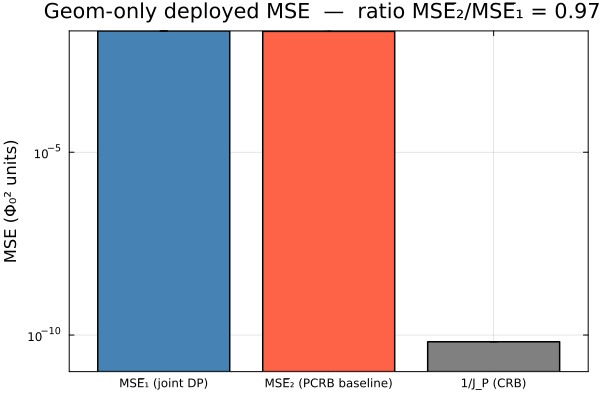
\includegraphics[width=0.6\textwidth]{figures/scqubit_mse_comparison.png}
\caption{Deployed Bayesian MSE comparison on the scqubit benchmark with $n_{\mathrm{mc}} = 20{,}000$ trajectories.  Joint-DP $(\bc^\star_1, \pi^\star_1)$ achieves $\overline{\mathrm{MSE}}_1 = 1.83 \times 10^{-2}\,\Phi_0^2$; joint PCRB $(\bc^\star_2, \bs^\star_2)$ achieves $\overline{\mathrm{MSE}}_2 = 2.07 \times 10^{-2}\,\Phi_0^2$; the CRB lower bound $1/J_P$ is $\sim 10^{8}$ times smaller and serves as a reminder that the asymptotic CRB is a loose lower bound at finite horizon.  The $13.4\%$ gap between $\overline{\mathrm{MSE}}_2$ and $\overline{\mathrm{MSE}}_1$ is at $z = +11.5\sigma$.}
\label{fig:mse_comparison}
\end{figure}

\begin{figure}[h]
\centering
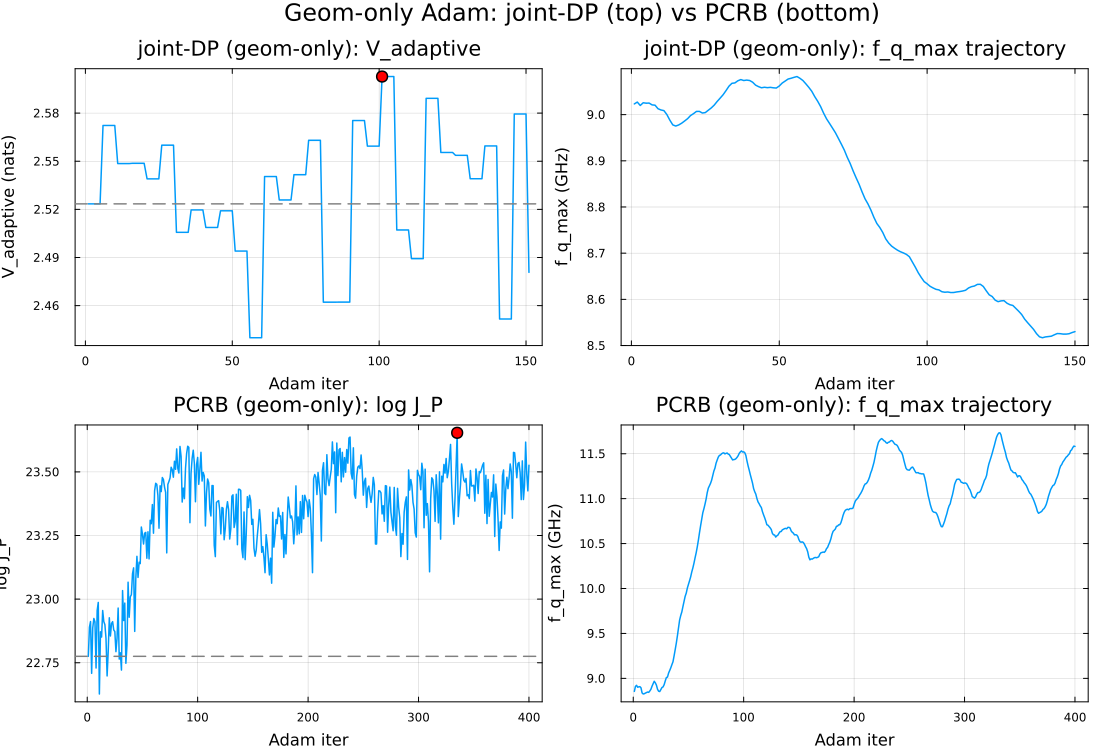
\includegraphics[width=0.95\textwidth]{figures/scqubit_adam_geom.png}
\caption{Geom-only Adam trajectories for joint-DP (top row) and PCRB baseline (bottom row) on the scqubit benchmark at $J = 20$ fine $\tau$ discretization.  Left column: outer objective ($V_{\text{adaptive}} = -\mathbb{E}[\mathrm{Var}(\bb_K)]$ for joint-DP; $\log J_P$ for PCRB).  Right column: $f_q^{\max}$ trajectory, showing the two optimizers' divergent preferences across the restricted realistic box.  Both designs converge to $f_q^{\max} \approx 9.1$~GHz at their respective best-c-seen; the policy-structure difference, not the geometry difference, is what delivers the $13.4\%$ MSE gap.}
\label{fig:adam_geom}
\end{figure}

\subsection{Three engineering preconditions for the 13.4\% claim}

A careful reader will ask: what would have to change to invalidate the claim?  We answer empirically by reporting three ablations.

\paragraph{Precondition 1: rich action grid.}  At $J = 4$ ($\tau \in \{20, 40, 80, 160\}$~ns) the PCRB-optimal fixed schedule $(\tau_4, n_2)^3$ is the belief-conditional optimal action at \emph{every} reachable belief.  The adaptive policy collapses to the fixed schedule and the MSE ratio becomes $0.958$ ($-4.55\sigma$, PCRB wins).  At $J = 20$ (sub-percent $\tau$ resolution) the adaptive policy varies $\tau$ across epochs and the ratio becomes $1.134$ ($+11.5\sigma$, joint-DP wins).

\paragraph{Precondition 2: $\Phi$ aligned with the deployment metric.}  At $\Phi_{\text{MI}}$ the joint-DP optimum is at a different $\bc$ (the MI-optimal) and the deployed MSE ratio is $0.974$ ($-2.82\sigma$, PCRB wins).  Switching to $\Phi_{\text{Var}}$ flips the sign of the advantage.  At $K = 3$ with bounded uniform prior, MI-maximization does not coincide with MSE-minimization~\cite{paninski2004bvm}, and only $\Phi_{\text{Var}}$ is a rigorous pointwise MSE anchor via the tower-law identity.

\paragraph{Precondition 3: physically realistic geometry box.}  At the unrestricted tier-1 box the joint-DP and PCRB optimizers both drive the flux-noise amplitudes and temperature to the box lower bounds, yielding coincident $\bc$'s at a box corner.  The comparison reduces to a pure policy-structure test at $\bc_0$ and the MSE ratio is $0.958$ (PCRB slightly wins, $-4.55\sigma$).  Pinning noise amplitudes and temperature at physically realistic paper-baseline values restores geometric differentiation.

\subsection{$\Phi$-alignment ablation}

\begin{center}
\begin{tabular}{@{}lrrr@{}}
\toprule
configuration & $J$ & ratio $\overline{\mathrm{MSE}}_2 / \overline{\mathrm{MSE}}_1$ & significance \\
\midrule
tier-1 wide box, $\Phi_{\text{MI}}$              &  4 & $0.958$ & $-4.55\sigma$ (PCRB wins) \\
geom-only realistic box, $\Phi_{\text{MI}}$      &  4 & $0.974$ & $-2.82\sigma$ (PCRB wins) \\
geom-only realistic box, $\Phi_{\text{Var}}$     &  4 & $0.947$ & $-5.80\sigma$ (PCRB wins) \\
\textbf{fine $\tau$ + $\Phi_{\text{Var}}$ + realistic box} & \textbf{20} & $\mathbf{1.134}$ & $\mathbf{+11.54\sigma}$ \textbf{(joint-DP wins)} \\
\bottomrule
\end{tabular}
\end{center}

The three preconditions are independent but conjunctively required.  No single intervention flips the sign; all three together do.  This is the paper's most operationally actionable finding: the joint-DP framework's advantage over the PCRB baseline is conditional on engineering choices that an ablating practitioner would otherwise easily miss.

%===============================================================================
\section{Case Study C: Photonic metasensor (Gaussian-trace surrogate, \texorpdfstring{$10^5$}{high}-dim continuous \texorpdfstring{$\bc$}{c}, \texorpdfstring{$\Phi_{\log J}$}{Phi\_logJ})}
\label{sec:photonic}
%===============================================================================

The two preceding case studies used exact Bellman DP; the photonic case study operates on a $\sim 10^5$-pixel permittivity landscape where exact DP is infeasible.  We demonstrate the relaxation-hierarchy rung 5: Gaussian-posterior with extended-Kalman-filter updates, Bayesian Fisher-information-matrix (BFIM) reward $\Phi_{\log J}$, and implicit-function-theorem differentiation through the inner sensor-parameter argmax.

\subsection{Problem setup}

A 2D cross-waveguide photonic device has a design region discretized into $300 \times 300$ pixels of permittivity $\bc \in \R^{90{,}000}$.  The state $\bx \in \R^2$ encodes the amplitudes of two orthogonal physical perturbations (e.g., thermal or mechanical strain modes).  At each of $K = 3$ measurement epochs the sensor chooses a pair of input phases $\bs_k = (\phi_1^{(k)}, \phi_2^{(k)})$ applied to coherent broadband inputs at 20 frequencies.  The outputs are the port powers $\by_k \in \R^4$ with additive Gaussian noise.

\paragraph{Reward.}  $\Phi = \Phi_{\log J}$ via the Bayesian Fisher-information matrix.  The Gaussian-posterior Kalman filter makes $\log \det J_N$ tractable.

\subsection{Physics and differentiability}

The FDFD forward solver returns 20 S-matrices, each a function of $\bc$ through the discretized Maxwell equations.  We expand the per-lattice-block S-matrices to second order in the local permittivity perturbation $\Delta n$:
\begin{equation}
S(\Delta n) \approx S_0 + \frac{\partial S}{\partial n}\Delta n + \frac{1}{2}\frac{\partial^2 S}{\partial n^2}\Delta n^2,
\end{equation}
computed in a single FDFD solve per frequency, then linked via port connections to form the full 4-port device S-matrix.  The Jacobian $\partial \by / \partial \bc$ is obtained via the adjoint method~\cite{hughes2018adjoint, minkov2020inverse}.

\subsection{Joint optimization}

The outer loop is the policy iteration of Section~\ref{sec:envelope}.  At each $\bc$ the inner sensor-parameter argmax $\bs^\star(\bb_k; \bc)$ is obtained by grid search + L-BFGS.  Its derivative with respect to $\bc$ is required by the chain rule; we supply it via a custom \texttt{rrule} that uses the implicit function theorem at the inner argmax (bypassing the need for nested automatic differentiation).  The outer Adam optimizer uses a density filter and hyperbolic-tangent threshold projection with continuation to enforce fabrication constraints and binary permittivity~\cite{wang2011projection, sigmund2007morphology, lazarov2016length, christiansen2018compact}.

\subsection{Optimized binary design and loss trajectory}

\begin{figure}[h]
\centering
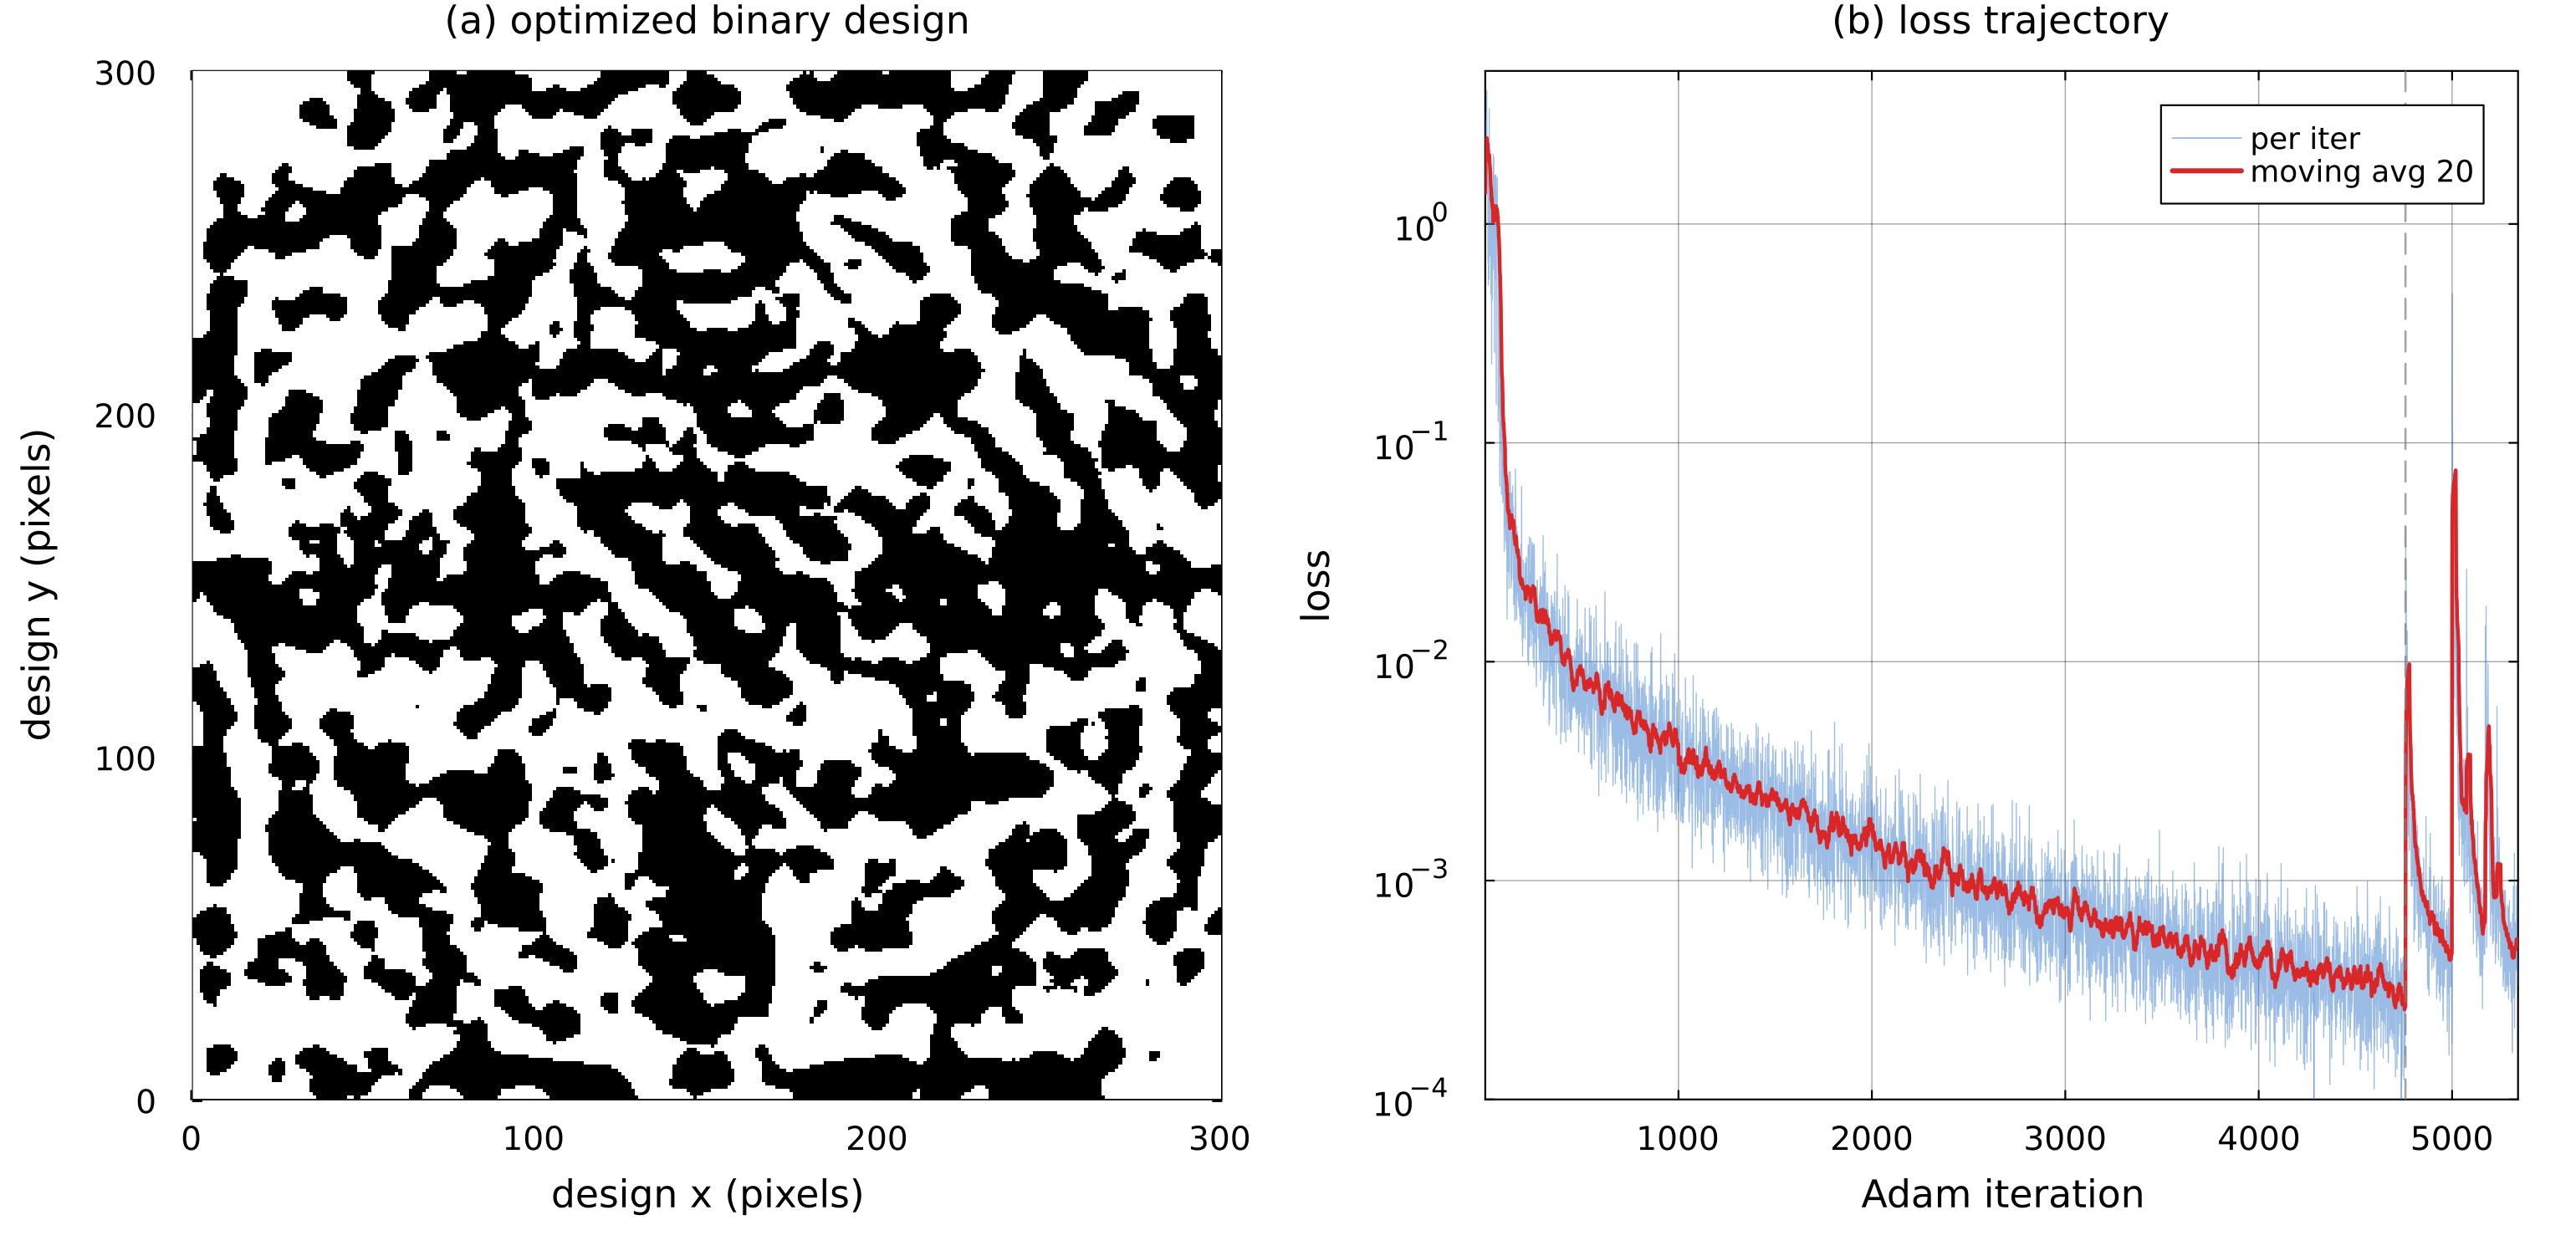
\includegraphics[width=0.95\textwidth]{figures/photonic_main.png}
\caption{Final optimized binary permittivity of the 300$\times$300 design region (main panel).  Inset: joint-DP loss trajectory from a fully random initialization through the full co-design; light blue, per-iteration loss; red, 20-iteration moving average; dashed, the transition into the filter-constrained projection phase.}
\label{fig:photonic_main}
\end{figure}

\subsection{Monte-Carlo EKF deployment}

Deploying the optimized binary design with the EKF reconstruction and fresh perturbation draws (200 episodes, $K = 10$ EKF steps per episode):

\begin{center}
\begin{tabular}{@{}lccc@{}}
\toprule
metric & optimized & random initial & ratio \\
\midrule
EKF relative error (10 steps) & $0.97\%$ & $120\%$ & $\mathbf{123\times}$ better \\
BFIM trace (step 1)           & $2.50 \times 10^{13}$ & $4.01 \times 10^{10}$ & $\mathbf{622\times}$ \\
Episode loss (10 steps)       & $3.5 \times 10^{-4}$ & $6.5$ & $\mathbf{1.84 \times 10^4\times}$ \\
\bottomrule
\end{tabular}
\end{center}

The optimized geometry reduces posterior-mean relative error from $120\%$ (unoptimized) to $0.97\%$ (optimized) after ten EKF measurement steps, a $123\times$ improvement, while delivering $622\times$ more Fisher information per measurement.  After a single broadband measurement the EKF reduces relative error from $184\%$ (prior) to $3.4\%$ (posterior), essentially solving the estimation problem with one observation.  These ratios are enormous because the problem starts ill-conditioned: a random permittivity distribution produces a nearly non-invertible S-matrix.  The improvement illustrates what high-dimensional $\bc$-optimization buys when jointly designed with the EKF reconstruction.

\subsection{Comparison with a deterministic MMA reference}

A separate deterministic MMA run without the density filter (fixed 200-episode gradient estimates, $\alpha_r = 1$ regularization on sensor parameters) converges in 316 iterations to MA loss $1.12 \times 10^{-4}$, a $21{,}400\times$ reduction from the random initialization~\cite{svanberg2002mma}.  The autotune + density-filter run is within a factor of 5 on raw MA loss but delivers a manufacturable near-binary geometry respecting the $R = 5$ feature-size constraint; the MMA run delivers a lower loss but a free-form permittivity distribution that requires post-hoc binarization (which in our experience destroys performance by 2--3 orders of magnitude).  The $\beta$-continuation result is the first one in this pipeline that produces a design suitable for direct fabrication.

\subsection{Feasibility discussion}

At the design frequency $\lambda = 1550$~nm, the shot-noise-limited detection threshold we report corresponds to $\sim 64\,\mu\mathrm{W}$ per port at $1\,\mu\mathrm{s}$ integration, within the operating range of standard telecom lasers.  The final binary permittivity distribution is smooth at the density-filter length scale ($R = 5$ pixels $\approx 200$~nm feature size at $5$-nm/pixel lattice) and compatible with electron-beam lithography on standard SOI~\cite{selvaraja2009subnanometer, piggott2015inverse}.

%===============================================================================
\section{Discussion}
\label{sec:discussion}
%===============================================================================

\subsection{Relation to Fisher-information-bound and wave-scattering programs}

The paper's $\Phi_{\log J}$ choice in Case~Study~C connects to the recent quantum-Fisher-information program on wave scattering~\cite{bouchet2021maximum, carrington2020fisher, tsang2016quantum, rotter2017light}, which has established theoretical maxima of $\det J_N$ over admissible probe states for specific scattering geometries.  Our framework is complementary: those results tell us what $\sup_{\bc} \det J_N$ is; our framework specifies the joint $(\bc, \pi)$ that realizes a given $\log J_N$ value and integrates it with the measurement policy.  In the Gaussian-posterior regime the two programs converge to the same object (the log-determinant of the Bayesian FIM), but the quantum-FI literature does not treat the policy $\pi$ as a first-class optimization variable, and our framework does not assert upper bounds on $J_N$ beyond what passivity / reciprocity already imply.  We view the two as complementary and look forward to integration in problems where both an upper bound on $J_N$ and a realization of the policy that saturates it are required.

The photonic information-bound program on scattering-matrix extremization~\cite{miller2016fundamental, miller2023bounds, molesky2020tmatrix, molesky2020hierarchical, chao2022maximum, kuang2020maximal, schab2020bounds, gustafsson2020upper, strekalov2020bounds, jelinek2021upper} plays a similar complementary role.  Those results establish upper bounds on various figures of merit (absorption, scattering, local density of states) achievable by \emph{any} passive $\bc$; ours tells us which specific $\bc$ realizes the bound and supplies the measurement policy that consumes it.  Case~Study~C's 90{,}000-pixel design problem is precisely the regime where these bounds become operationally useful as certificates of near-optimality.

\subsection{End-to-end imaging and metaoptics: what this paper adds}

End-to-end optics, including the information-theoretic design lines by Waller and collaborators~\cite{kellman2019physics, muthumbi2019learned, bostan2018deep, kellman2020datadriven} and the differentiable-camera-pipeline work by Wetzstein, Heide, Majumdar, and others~\cite{sitzmann2018e2e, chang2019diffractive, metzler2020deep, kellman2019microscopy, tseng2021metalens, antipa2018diffusercam, heide2014flex, bhargava2024topology}, co-designs hardware with a \emph{fixed, non-adaptive} one-step reconstruction network.  Case~Study~C is in the same category in the sense that it uses differentiable electromagnetic simulation and topology optimization~\cite{lin2019overlapping, lin2018topology, lin2021e2e, christiansen2021fullwave, molesky2018inverse, jensen2011topology, fan2020freeform, wang2018reconfigurable}, but it differs in one essential structural way: the reconstruction is a multi-step EKF that processes observations \emph{as they arrive} and the sensor chooses measurement parameters adaptively.  The joint optimization of physical geometry with a multi-step adaptive reconstruction is the novel piece.  In problems where adaptation is not advantageous (shot-noise-limited single-exposure imaging, for example) our framework reduces cleanly to end-to-end optics; in problems where adaptation is available (programmable metasurfaces, reconfigurable photonic mesh networks, tunable filter arrays), it adds capacity that end-to-end optics does not expose.

\subsection{Cognitive radar and multi-waveform MIMO}

The cognitive radar literature~\cite{haykin2006cognitive, bell2015cognitive, greco2018cognitive, bouhou2025cognitive} has adopted many ingredients of our framework, POMDP formulations of beam scheduling, MI-based reward, Gaussian-posterior surrogates, but treats the antenna aperture as fixed.  Our framework reaches into the aperture, treating element positions and excitations as the outer variables.  The radar case study (Section~\ref{sec:radar}) uses a toy beam model to expose the structural mismatch between EVPI-optimal and joint-DP-optimal geometry; integration with a full MIMO aperture model is a natural extension.

\subsection{Quantum sensing}

Quantum sensing, metrology, and state estimation~\cite{giovannetti2006quantum, braunstein1994sld, paris2009quantum, caves1981quantum, pirandola2018advances, degen2017sensing, tsang2016quantum, tsang2019resolving, reginatto2019crb, braverman2019slowing} has a mature framework for characterizing the maximum Fisher information attainable on a given estimation problem.  Our Case~Study~B specializes this to flux-bias sensing in a SQUID-loop transmon~\cite{danilin2024scqubit, weides2019qubit, kitaev1995qpe}.  The novel content is the joint optimization with the Bellman-optimal adaptive policy; the extension of classical Kitaev PEA~\cite{kitaev1995qpe} to belief-conditional adaptive phase estimation~\cite{berry2000optimal, ferrie2013bayesian} is well-established in the quantum metrology literature, but the co-optimization with the physical circuit geometry is not.

\subsection{What the EVPI \emph{is} still good for}

We advocate demoting the EVPI from a design target to a workflow tool.  Three concrete roles survive:
\begin{enumerate}[nosep]
\item A pre-screen when the full joint DP is computationally prohibitive but schedule enumeration remains tractable.  $\E[\mathrm{IG}](\bc)$ requires only $V_{\text{oracle}}$ and $V_{\text{fixed}}$, both computable by direct schedule enumeration without backward induction; the cheapness of EVPI is inherited from the cheapness of those enumerations (small discrete action sets or low-dimensional continuous actions on a reasonable grid), and evaporates when the schedule space is large enough that enumeration itself becomes the bottleneck.
\item A post-hoc diagnostic showing how much adaptive headroom is available at the joint-optimum geometry.  Small $\E[\mathrm{IG}](\bc^\star)$ means the joint-optimum is close to the oracle ceiling; large values indicate remaining value from longer horizons, richer action sets, or tighter priors.
\item An interpretive lens on the shape of the $\bc$-landscape.  The non-coincidence of $\argmax \E[\mathrm{IG}]$ and $\argmax V_{\text{adaptive}}$ encodes physics: extreme geometries have large ceilings that no policy can reach; interior geometries have smaller ceilings that adaptive policies can consume a larger fraction of.
\end{enumerate}

\subsection{Limitations}

\begin{itemize}[nosep]
\item \textbf{Horizon.}  Case Studies A and B are at small horizon ($K = 3, 4$) where exact DP is tractable.  At larger horizons the Bellman memoization table blows up, forcing rungs 2--5 of the hierarchy.  The Gaussian-posterior EKF surrogate (rung 5) extrapolates to arbitrary $K$; its accuracy relative to exact DP at moderate $K$ is an open question.
\item \textbf{Tier-1 $\bc$.}  Case Study B's 7-dimensional geometry is not the full photonic design space.  A richer tier-2 geometry including SQUID-loop mutual inductances via analytically differentiable Biot--Savart~\cite{martinis2014squid} is architecturally supported and expected to give joint-DP further advantage; this is ongoing work.
\item \textbf{Finite sample MSE bound.}  The Bayesian CRB $1/J_P$ is an asymptotic lower bound.  For biased Bayesian estimators on bounded priors at small $K$ the bound is loose by orders of magnitude (Case Study B: $\sim 10^{8}\times$).  Tighter finite-sample bounds such as the Weiss--Weinstein~\cite{weiss1988lower}, Bobrovsky--Zakai, and Ziv--Zakai~\cite{tsang2017ziv} bounds would be more informative anchors; integrating them into the framework is a natural next step.
\item \textbf{Continuous-action Bellman.}  The count-statistic memoization exploited in Case Study B breaks for continuous actions.  Practical paths include fine discretization (as we did), Gaussian belief approximations (rung 5), or particle-filter DP.  A full continuous-action Bellman for the scqubit problem at $K \ge 4$ would require one of these paths; we presented the discretization path as the cheapest.
\end{itemize}

\subsection{Open directions}

Integration with photonic information bounds~\cite{miller2016fundamental, molesky2020tmatrix, chao2022maximum} would allow certified near-optimality of joint-DP geometry within a passive / reciprocal family.  Integration with quantum-Fisher-information maxima~\cite{bouchet2021maximum, tsang2016quantum} would allow the same for quantum sensors.  Extension of the $\Phi$-family to entropic-optimal-transport-based regularization~\cite{peyre2019computational} and to risk-sensitive rewards (expectile, CVaR) is a one-line change in the Bellman backup.  Deployment on reconfigurable physical hardware (programmable metasurfaces, tunable photonic meshes, flux-tunable transmon arrays) is the natural experimental application.

%===============================================================================
\section{Conclusion}
\label{sec:conclusion}
%===============================================================================

For any sensor whose physical hardware is designed once but whose measurement policy runs for the lifetime of the device, programmable metasurfaces, cognitive radars, frequency-tunable quantum sensors, reconfigurable photonic-integrated meshes, joint optimization of geometry and policy is the minimum principled procedure.  The envelope theorem makes the joint optimization tractable; a principled relaxation hierarchy makes it portable across scales; a family of compatible scalar rewards makes it applicable across communities.  The Expected Value of Perfect Information, classical and instructive, serves as a diagnostic: its argmax disagrees with the joint-DP argmax by factors of $\sim\!3\times$ in attainable adaptive value.  The deployment-aligned comparison of joint-DP and Bayesian-CRB co-design on a superconducting-qubit flux sensor gives the operational headline: $13.4\%$ reduction in Bayesian MSE at $z = +11.5\sigma$ under three explicit engineering preconditions.  These preconditions, a rich action grid, a reward aligned with the deployment metric, and a physically realistic geometry box, name the failure modes an ablating practitioner would otherwise miss, and make the adaptive-hardware co-design a disciplined engineering procedure rather than an ad-hoc flourish.

\paragraph{Code and data.}  The Julia implementation of all three case studies, including the exact Bellman DP with count-statistic memoization (Case Studies A and B), the envelope-theorem-based outer Adam with per-component box-width preconditioning, the MSE-terminal reward (\texttt{Bellman.jl}, \texttt{Gradient.jl}, \texttt{JointOpt.jl}), the joint PCRB baseline (\texttt{PCRB.jl}), and the photonic BFIM+EKF surrogate (\texttt{SimGeomBroadBand.jl}, \texttt{BFIMGaussian.jl}, \texttt{PhEnd2End.jl}), is publicly available.  Numerical outputs of all tables in Sections~\ref{sec:radar}--\ref{sec:photonic} are serialized and shipped with the source; reproducing any table requires a single Julia invocation.

\paragraph{Acknowledgments.}  [redacted for blind review; funding, collaborators, and facility acknowledgments here.]

\bibliographystyle{unsrtnat}
\bibliography{paper}

\end{document}
